%%======%%======%0%======%%=======%%
\vspace{5mm}
\section{Decisões de UI/UX}


%%======%%======%0%======%%=======%%
\subsection{Interface e Experiência do Usuário}

O desenvolvimento da interface do sistema foi orientado mediante tudo postulado acima, a fim de organizar
as informações e funcionalidades do lab. de maneira intuitiva para todos.

\subsubsection{User Interface (UI)}

A construção da interface visual foi baseada na busca por consistência entre
as diferentes páginas do sistema. Para isso, os estilos foram modularizados
em diferentes arquivos CSS, responsáveis por funções específicas. O arquivo
\texttt{reset.css} estabelece uma base de normalização dos elementos,
enquanto \texttt{variables.css} concentra propriedades visuais reutilizáveis.
Os arquivos \texttt{base.css}, \texttt{layout.css} e
\texttt{components.css} são utilizados, respectivamente, para estilos
fundamentais, organização estrutural das páginas e definição dos componentes
visuais da interface.

Essa organização permite estabelecer uma linguagem visual compartilhada
entre as diferentes páginas, reduzindo inconsistências e facilitando a
manutenção do código. Componentes como botões, cartões, campos de formulário
e elementos de navegação podem, dessa forma, seguir padrões visuais
semelhantes independentemente da página em que são utilizados.

A utilização de variáveis CSS também contribui para a centralização das
decisões relacionadas à identidade visual. Dessa forma, alterações em
propriedades globais da interface podem ser realizadas de maneira
centralizada, evitando a necessidade de modificar individualmente cada
componente ou página.

Outro aspecto considerado foi a hierarquia visual. Títulos, subtítulos,
textos, botões e elementos informativos são organizados de maneira a
estabelecer diferentes níveis de importância. Essa hierarquia permite que o
usuário identifique inicialmente as informações mais relevantes e,
posteriormente, acesse conteúdos complementares. A figura abaixo evidencia a interface criada
\begin{figure}[H]
	\centering
	
	\begin{subfigure}{0.48\textwidth}
		\centering
		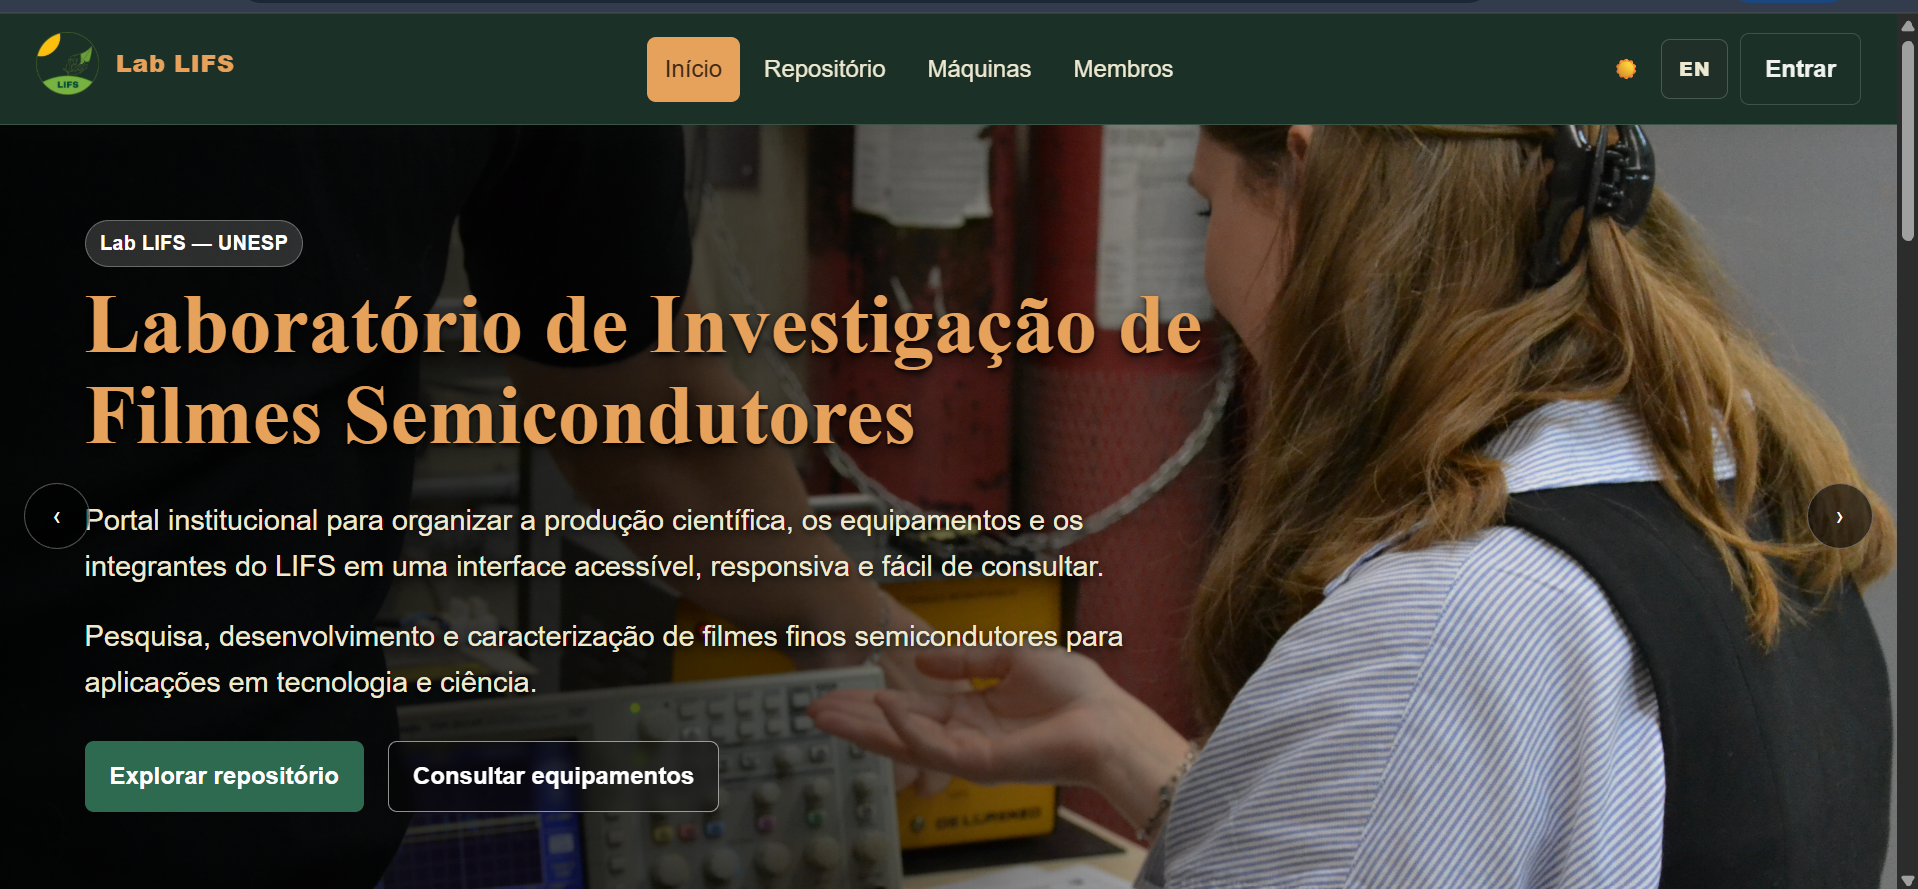
\includegraphics[width=\linewidth]{2-imagens/print_home_dark}
		\caption{Página inicial em tema escuro.}
		\label{fig:home-dark}
	\end{subfigure}
	\hfill
	\begin{subfigure}{0.48\textwidth}
		\centering
		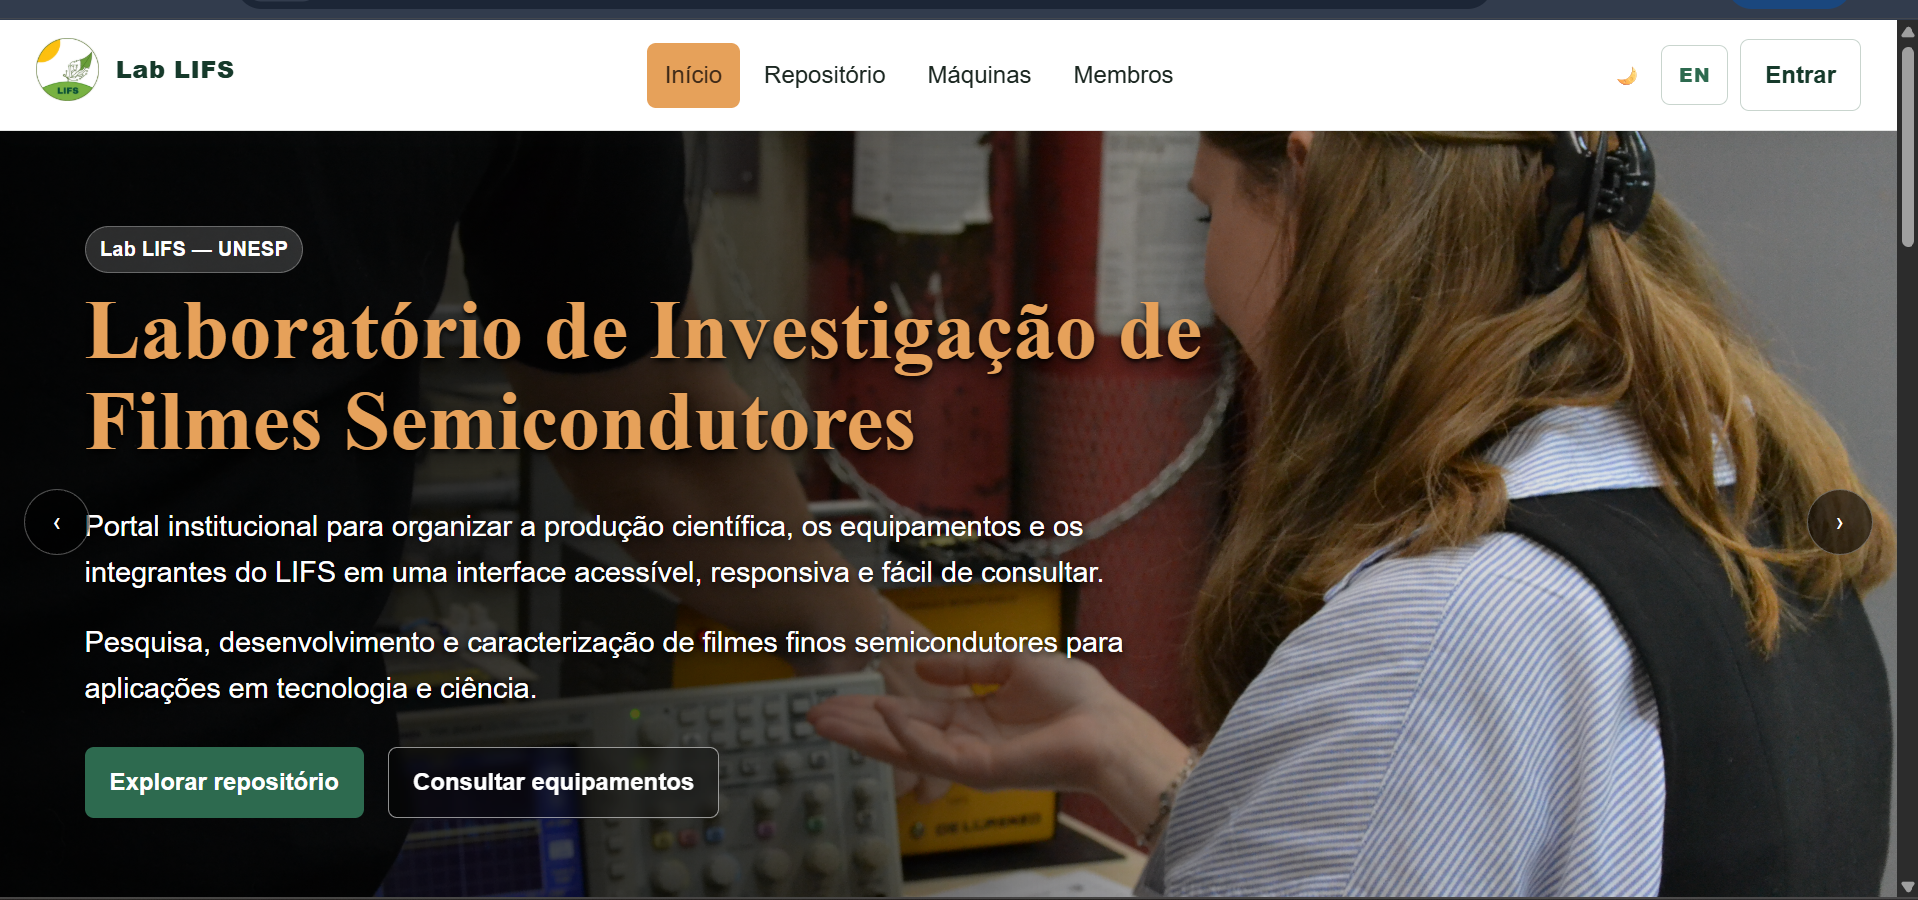
\includegraphics[width=\linewidth]{2-imagens/print_home_light}
		\caption{Página inicial em tema claro.}
		\label{fig:home-light}
	\end{subfigure}
	
	\vspace{0.5cm}
	
	\begin{subfigure}{0.48\textwidth}
		\centering
		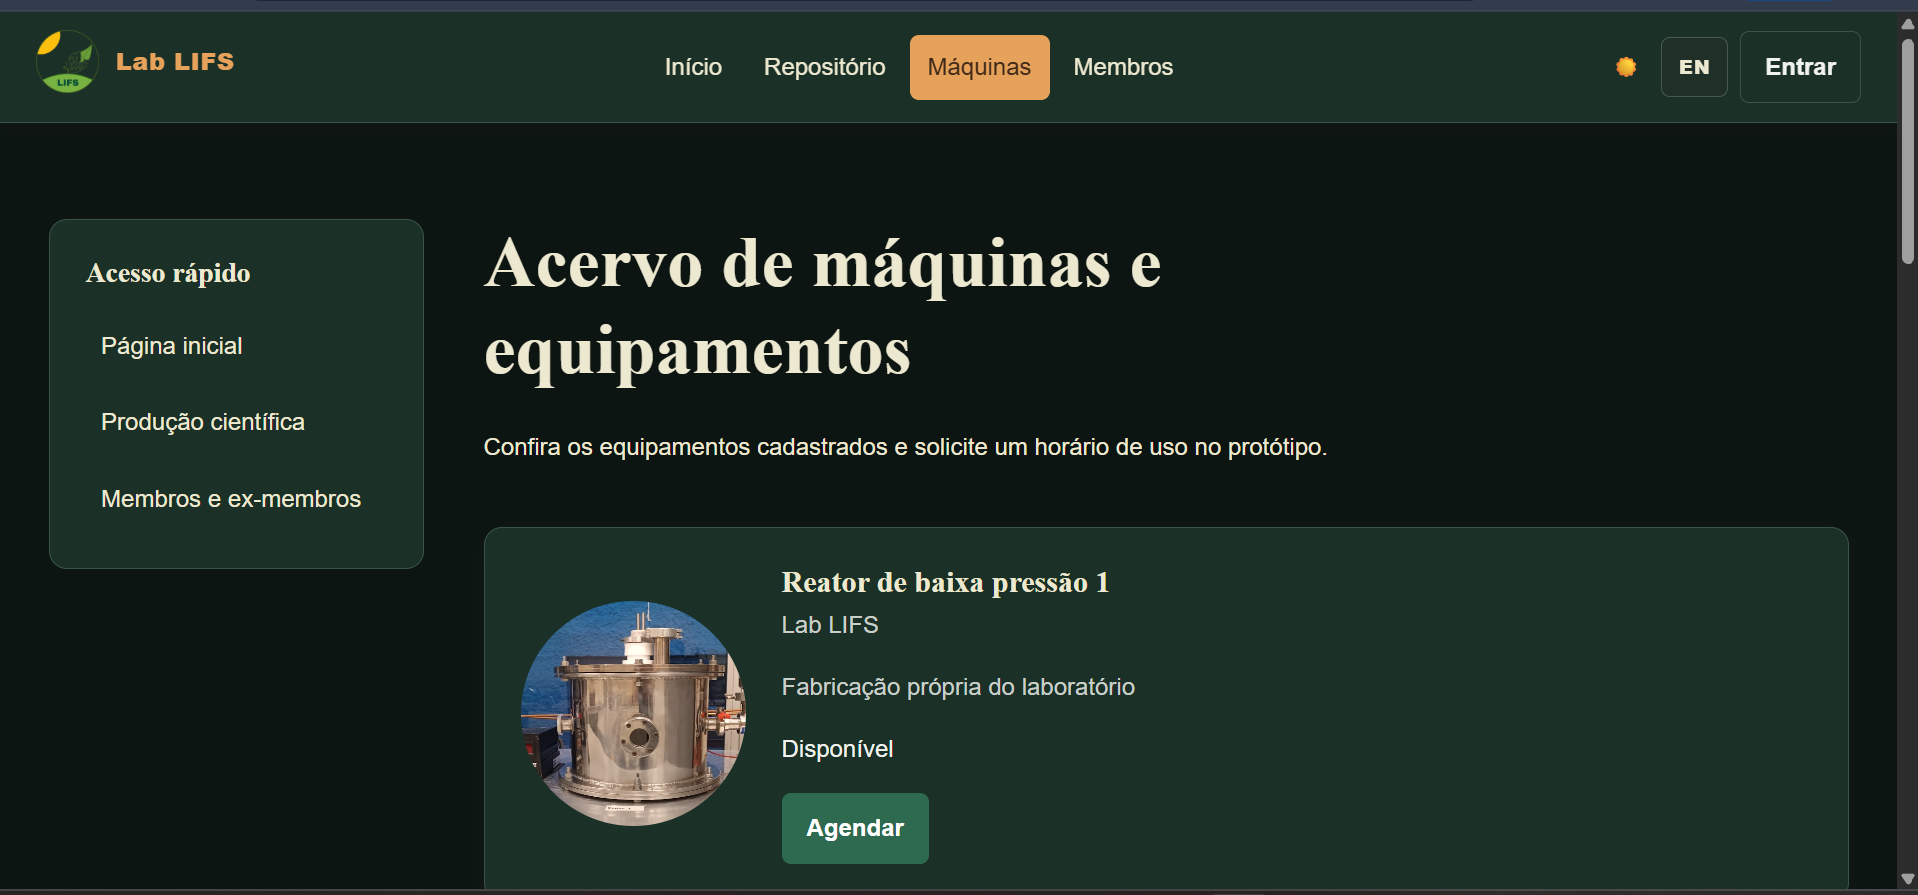
\includegraphics[width=\linewidth]{2-imagens/print_maq_dark}
		\caption{Página de máquinas em tema escuro.}
		\label{fig:maq-dark}
	\end{subfigure}
	\hfill
	\begin{subfigure}{0.48\textwidth}
		\centering
		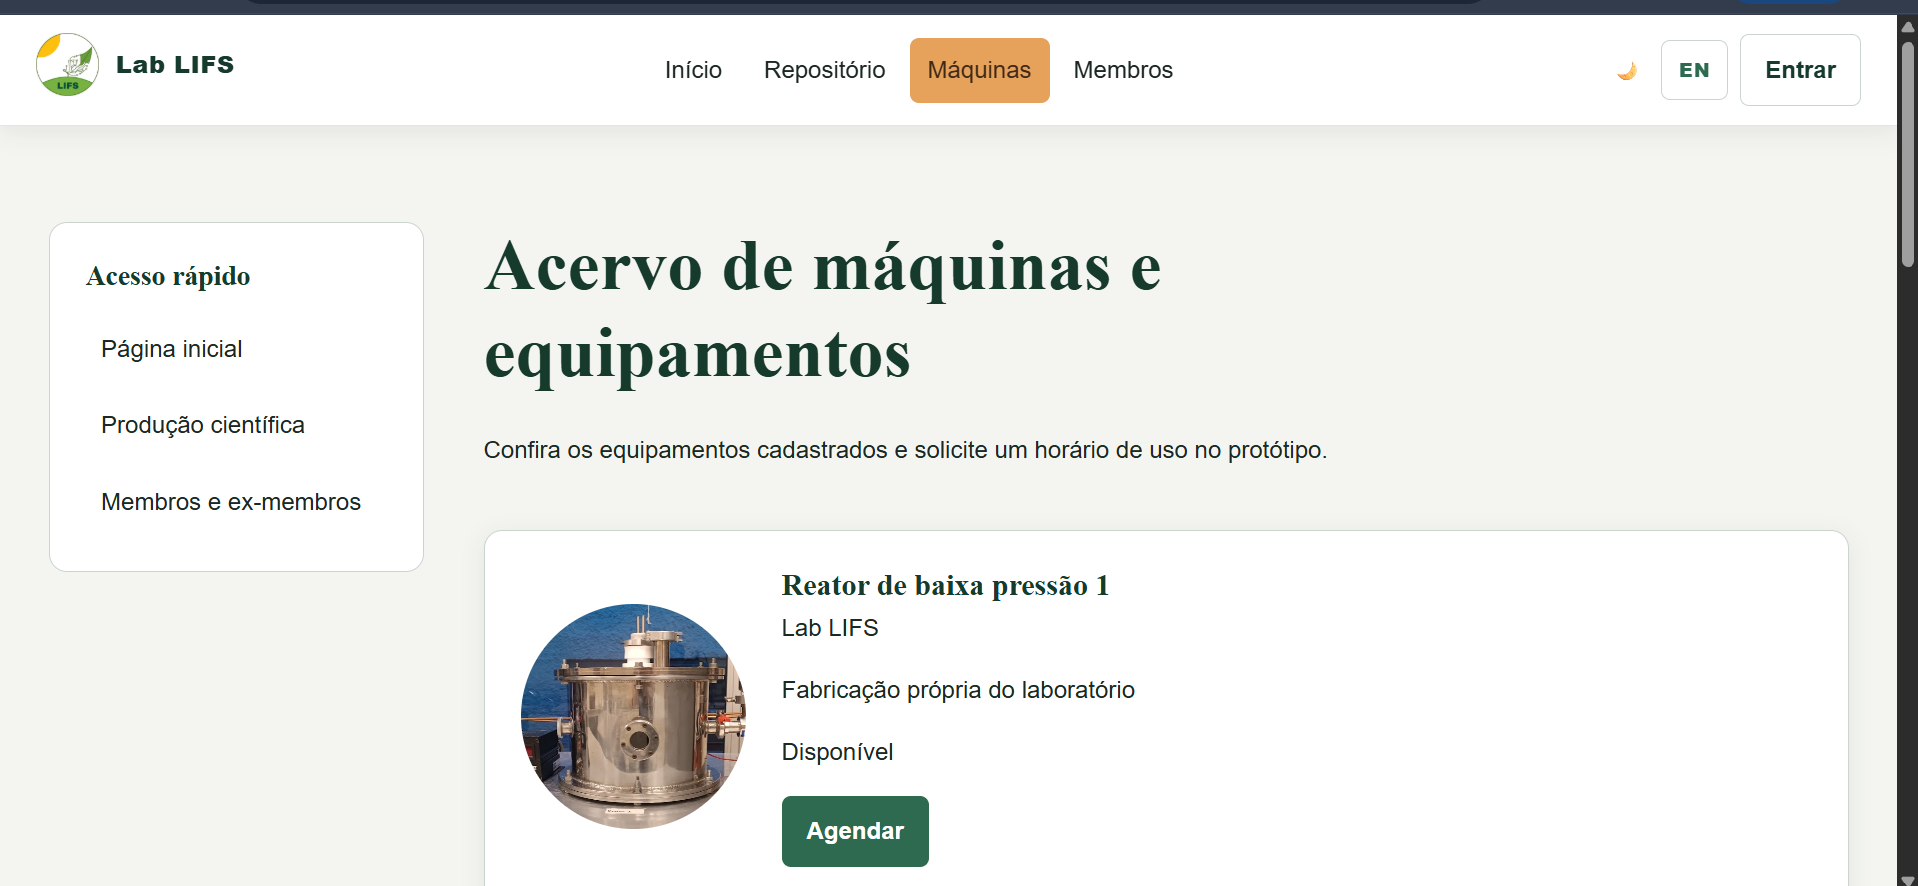
\includegraphics[width=\linewidth]{2-imagens/print_maq_light}
		\caption{Página de máquinas em tema claro.}
		\label{fig:maq-light}
	\end{subfigure}
	
	\caption{Interface do sistema nas páginas inicial e de máquinas, 
		apresentando os temas claro e escuro.}
	\label{fig:interface-temas}
\end{figure}

\subsubsection{User Experience (UX)}

No âmbito da experiência do usuário, a estrutura do sistema foi organizada
a partir da forma como diferentes usuários podem buscar informações sobre um
laboratório de pesquisa. A navegação principal foi dividida em categorias
associadas a conceitos distintos do LIFS, como \textit{Início},
\textit{Membros}, \textit{Máquinas} e \textit{Repositório}.

Essa organização constitui uma forma de arquitetura da informação, na qual
os conteúdos são agrupados segundo sua finalidade e não segundo sua
implementação interna. Assim, um usuário interessado em identificar os
pesquisadores pode acessar diretamente a área de membros, enquanto um
usuário interessado na infraestrutura pode consultar a seção de máquinas.
De maneira semelhante, a produção científica pode ser acessada por meio do
repositório.

A estrutura pode ser representada conceitualmente da seguinte maneira:

\begin{figure}[H]
	\centering
	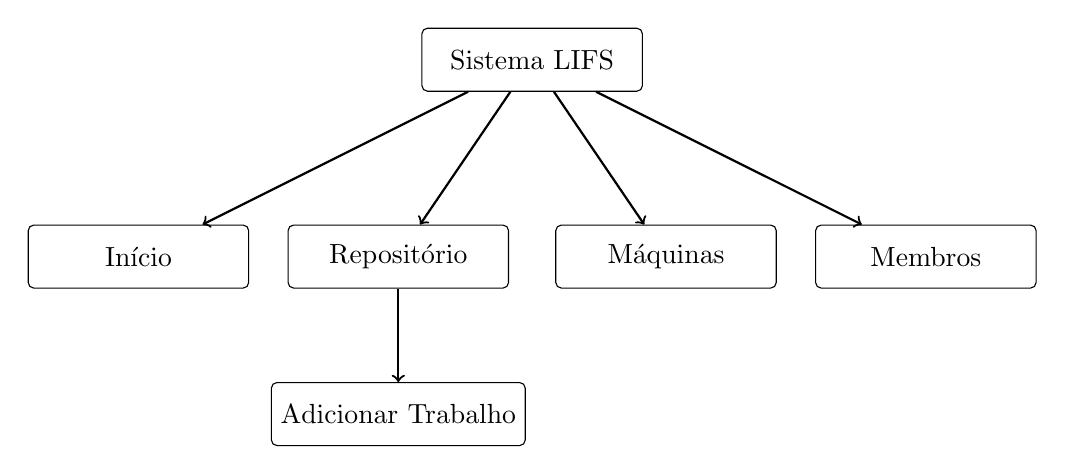
\begin{tikzpicture}[
		box/.style={
			draw,
			rounded corners=2pt,
			align=center,
			minimum width=2.8cm,
			minimum height=0.8cm
		},
		arrow/.style={
			->,
			thick
		}
		]
		
		% Sistema principal
		\node[box] (lifs) at (0,2.5) {Sistema LIFS};
		
		% Áreas principais
		\node[box] (inicio) at (-5,0) {Início};
		\node[box] (repo) at (-1.7,0) {Repositório};
		\node[box] (maquinas) at (1.7,0) {Máquinas};
		\node[box] (membros) at (5,0) {Membros};
		
		% Funcionalidade do Repositório
		\node[box] (adicionar) at (-1.7,-2) {Adicionar Trabalho};
		
		% Ligações principais
		\draw[arrow] (lifs) -- (inicio);
		\draw[arrow] (lifs) -- (repo);
		\draw[arrow] (lifs) -- (maquinas);
		\draw[arrow] (lifs) -- (membros);
		
		% Ligação do Repositório
		\draw[arrow] (repo) -- (adicionar);
		
	\end{tikzpicture}
	\caption{Organização hierárquica das principais áreas e funcionalidades do sistema LIFS.}
	\label{fig:arquitetura-lifs}
\end{figure}

Além disso, a presença de diferentes perfis de utilização foi considerada
na concepção do sistema. Um visitante externo pode utilizar a plataforma
principalmente para conhecer o laboratório e consultar suas informações,
enquanto um membro do grupo pode necessitar de funcionalidades adicionais,
como o cadastro de trabalhos. Essa diferenciação constitui uma base para a
evolução futura do sistema, especialmente para funcionalidades relacionadas
a autenticação, gerenciamento de conteúdo, disponibilidade de equipamentos e
agendamento.

\subsubsection{Fluxos de interação}

As funcionalidades do sistema também foram organizadas de maneira a
estabelecer relações entre consulta e execução de tarefas. Um exemplo é o
fluxo relacionado ao repositório científico, no qual o usuário pode acessar
os trabalhos disponíveis e, posteriormente, utilizar funcionalidades de
cadastro para inserir novas produções.

De forma conceitual, o fluxo pode ser representado como:

\begin{equation}
	\text{Repositório}
	\rightarrow
	\text{Consulta}
	\rightarrow
	\text{Seleção do trabalho}
	\rightarrow
	\text{Visualização}
\end{equation}

Para usuários autorizados, esse fluxo pode ser expandido para:

\begin{equation}
	\text{Autenticação}
	\rightarrow
	\text{Cadastro}
	\rightarrow
	\text{Validação}
	\rightarrow
	\text{Publicação}
\end{equation}

A mesma abordagem poderá ser aplicada futuramente ao gerenciamento dos
equipamentos. Nesse caso, uma possível evolução da experiência de uso seria
permitir que o usuário selecione um equipamento, consulte sua
disponibilidade, escolha uma data e horário e confirme uma solicitação de
uso. Dessa forma, a interface deixa de ser apenas um meio de apresentação
das informações e passa a atuar como uma camada de interação com os
processos do laboratório.

\subsubsection{Estados e feedback da interface}

Outro aspecto relevante para a experiência do usuário é o fornecimento de
feedback após a execução de ações. Operações como cadastro, alteração ou
exclusão de informações devem apresentar ao usuário um retorno indicando se
a operação foi concluída ou se ocorreu algum erro.

Da mesma forma, situações nas quais não existem dados cadastrados devem ser
representadas por estados vazios informativos, evitando que o usuário
interprete uma área vazia como falha do sistema. Por exemplo, quando não
existirem trabalhos cadastrados no repositório, a interface poderá informar
explicitamente essa condição e apresentar uma orientação sobre a ação que
pode ser realizada.

Esses mecanismos são importantes para estabelecer uma comunicação clara
entre o sistema e o usuário, reduzindo incertezas durante a utilização.

\subsubsection{Responsividade e consistência}

A experiência do usuário também deve ser preservada em diferentes tamanhos
de tela. A interface foi concebida utilizando recursos de CSS que permitem a
adaptação da disposição dos elementos conforme o espaço disponível,
possibilitando sua utilização em computadores, notebooks e dispositivos
móveis.
\begin{figure}[H]
	\centering
	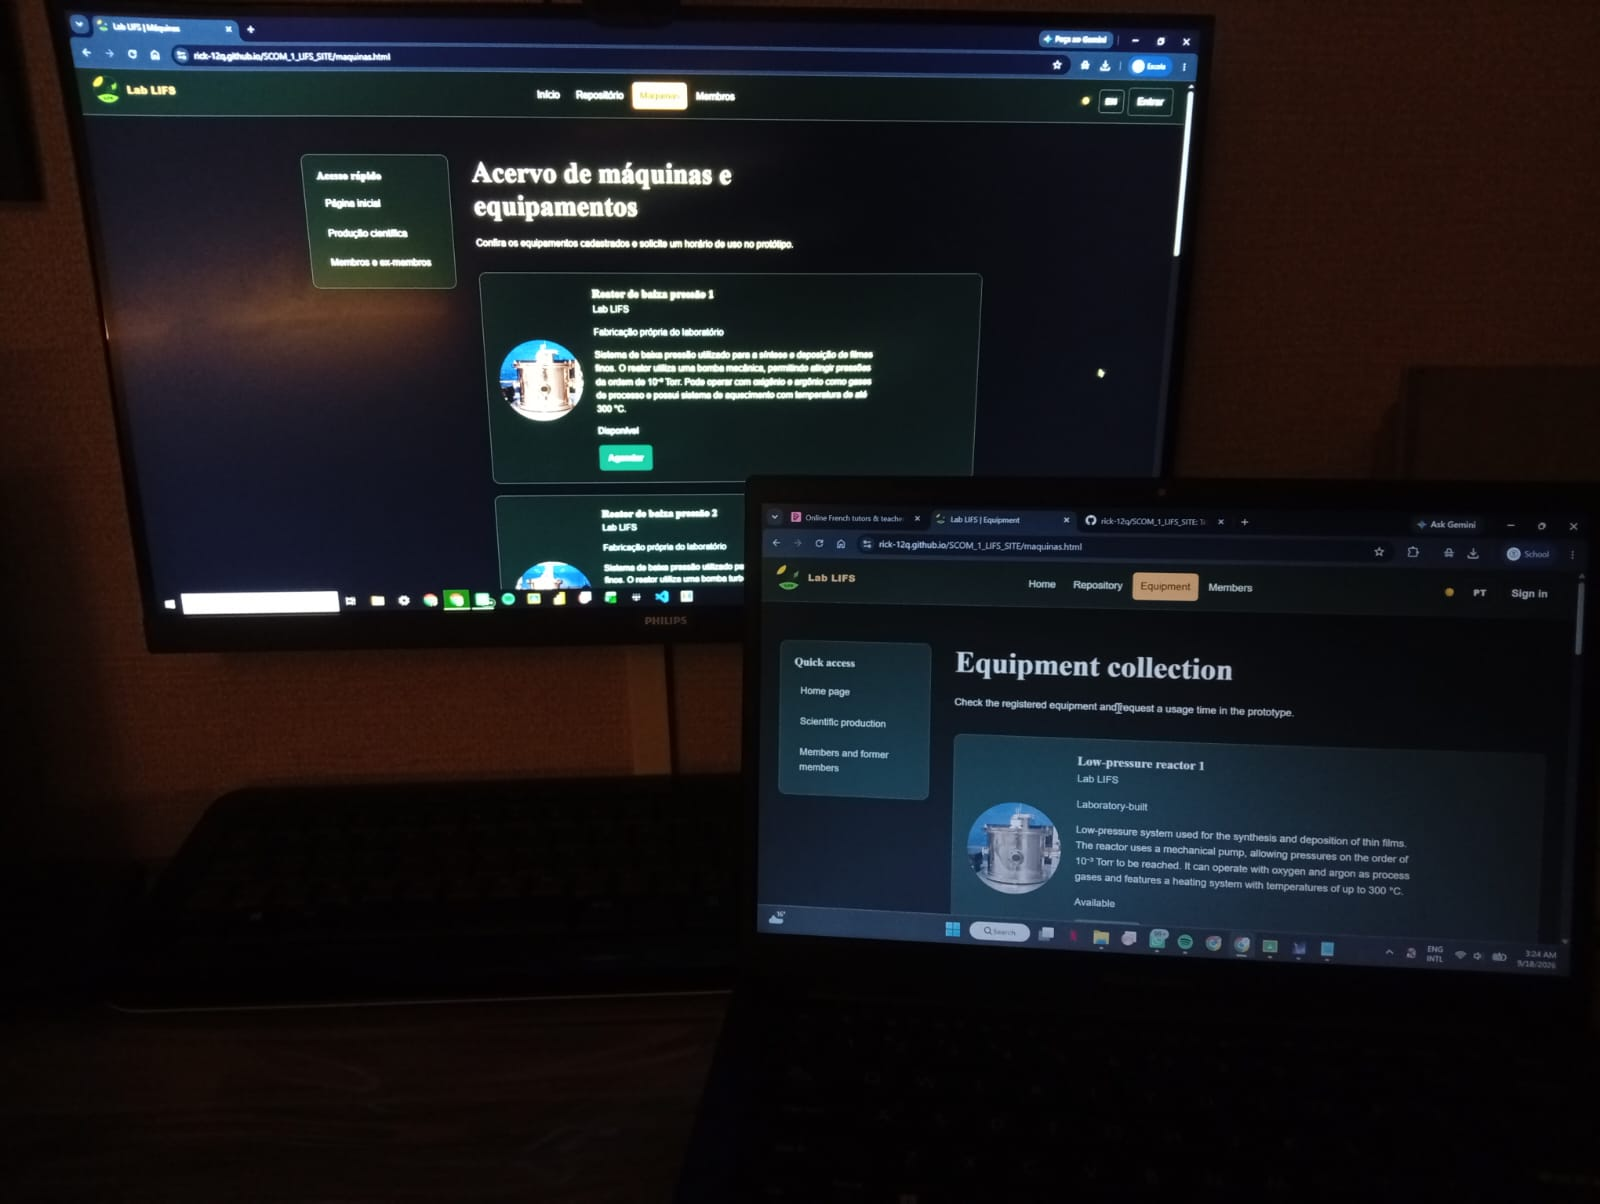
\includegraphics[width=0.7\linewidth]{2-imagens/telas-diferentes}
	\caption{Fotografia de duas telas com tamanhos visivelmente diferentes, enquadrando a mesma página do \textit{website}, evidenciando a responsividade. \\ \centering Fonte: O autor, 2026.}
	\label{fig:telas-diferentes}
\end{figure}

Nesse contexto, responsividade não é considerada apenas como a redução do
tamanho dos elementos, mas como a adaptação da hierarquia e da disposição
das informações. Em telas menores, elementos de navegação e componentes
visuais podem ser reorganizados para preservar sua legibilidade e
acessibilidade.

Dessa maneira, as decisões de UI e UX adotadas no sistema procuram
estabelecer uma relação entre identidade visual, arquitetura da informação e
facilidade de utilização. A interface constitui, portanto, não apenas uma
camada estética do projeto, mas também um mecanismo para organizar e tornar
acessíveis as informações e funcionalidades relacionadas ao LIFS.
